\documentclass{article}

% Encoding and Geometry
\usepackage[utf8]{inputenc}
\usepackage[a4paper, margin=1in]{geometry}
\usepackage{parskip}

% Math Packages
\usepackage{amsmath, amsfonts, mathtools}

% Graphics and Figures
\usepackage{graphicx}
\usepackage{caption}
\usepackage{subcaption}
\usepackage{multirow}
\usepackage{tikz}
\usetikzlibrary{positioning}

% Hyperlinks
\usepackage[colorlinks=true, linkcolor=blue, urlcolor=blue]{hyperref}

% Floating Objects Placement
\usepackage[section]{placeins}

% Bibliography
\usepackage[
backend=biber,
style=alphabetic,
sorting=ynt
]{biblatex}
\addbibresource{references.bib}

% Typesetting improvements
\usepackage{microtype}

% Title Information
\title{EulerSwap White Paper}
\author{Euler Labs}
\date{February 2025}

\begin{document}

\maketitle

\pagestyle{plain}

\begin{abstract}
Liquidity in decentralised exchanges (DEXs) is typically underutilised, with capital often sitting idle instead of earning yield elsewhere. EulerSwap addresses this inefficiency by integrating an automated market maker (AMM) with Euler's lending vaults. Liquidity providers (LPs) can earn swap fees, accrue lending yield, and borrow natively against their position. When a user initiates a swap, the AMM reuses collateral and debt within Euler to facilitate the trade and improve capital efficiency. If needed, EulerSwap can borrow the swap’s output token using the input token as collateral. This just-in-time (JIT) liquidity model can offer up to 50x greater liquidity depth than traditional AMMs by putting idle vault assets to more productive use. Unlike conventional AMMs that fragment liquidity across multiple pools, EulerSwap also improves capital efficiency by enabling a single, cross-collateralised vault to work as a liquidity hub to support many trading pairs simultaneously. It features a novel AMM design that enables asymmetric depth and concentrated liquidity—especially useful for new token launches. EulerSwap instances are modular, composable, and integrate natively with Uniswap v4 hooks, unlocking more flexible and programmable trading logic. By combining just-in-time liquidity, shared vaults across pools, and customisable AMM mechanics, EulerSwap reduces inefficiencies in liquidity provision—delivering deeper markets, lower costs, and greater control for liquidity providers.
\end{abstract}

\section{Introduction}

Liquidity on decentralised exchanges (DEXs) is often underutilised, sitting idle even when it could be generating additional yield elsewhere. This inefficiency raises costs for liquidity providers (LPs), limits market depth, and makes it harder for DEXs to compete with centralised platforms. EulerSwap addresses this by integrating an automated market maker (AMM) directly with Euler’s lending vaults, enabling liquidity to be used simultaneously for swaps, lending, and borrowing.

With EulerSwap, DEX reserves become dual-purpose. LPs can earn lending yield during periods of low trading activity and borrow against their liquidity to support deeper swap markets or use their capital productively elsewhere. This model significantly boosts capital efficiency and reduces opportunity cost.

Unlike traditional AMMs that pool liquidity from many LPs into a single contract, each EulerSwap instance is controlled by a single LP—an Euler account holder—who supplies both swap liquidity and collateral. When a user initiates a trade, EulerSwap can dynamically borrow the output token using the input token and the LPs' collateral as backing. This just-in-time (JIT) liquidity provision allows a relatively small amount of deposited capital to simulate much deeper liquidity. Under optimal conditions, \$1 million of initial collateral can support a swap market with the effective depth of a \$50 million AMM pool on a conventional DEX.

This model is especially valuable for new token projects, which often face high costs to bootstrap liquidity. Instead of seeding large pools upfront, they can create JIT-powered markets with deeper liquidity and lower capital requirements—while simultaneously establishing a lending market for their token.

EulerSwap also improves capital efficiency by allowing a single, cross-collateralised vault to act as a liquidity hub for multiple trading pairs. Similar in spirit to Curve’s 3pool, this design extends to any number of assets. For instance, one USDC vault on Euler could support swaps with USDT, USDe, DAI, USDS, RLUSD, and more—concurrently.

The protocol introduces a flexible AMM curve (see Figure \ref{fig:fig1}) that supports deep liquidity for short-term trading while helping to keep LPs' positions neutral over longer time horizons. LPs can customise pricing logic, apply asymmetric or single-sided liquidity strategies, and update their parameters by swapping out their EulerSwap operator contract (see below)—giving them far more control than pooled AMM models allow. This flexibility is particularly useful for professional market makers and token issuers who require precision in managing inventory and risk.

From the end-user perspective, EulerSwap delivers a seamless, Uniswap-style interface. Behind the scenes, it leverages innovations like JIT liquidity, shared vaults across pools, and customisable AMM mechanics—delivering deeper markets, lower costs, and greater control for liquidity providers. For DAOs, token projects, or market makers—EulerSwap offers a powerful tool for unlocking capital efficiency by uniting swap and lending markets in one modular, composable, and customisable system.

\section{Just-in-time (JIT) liquidity}

Under the hood, JIT liquidity works by leveraging the unique \texttt{operator} functionality of the Ethereum Vault Connector (EVC), a core immutable primitive at the heart of Euler. EVC operators allow Euler users to delegate authority over their account balances to a smart contract. An EulerSwap operator is a specialised contract that manages an LP’s account, rebalancing collateral and debt to support swaps and earn swap fees.

Consider the following example.

Suppose that Euler supports borrowing USDT with USDC as collateral at a loan-to-value (LTV) ratio of 0.95, and vice versa. This means that for every \$1 of USDC or USDT collateral, a user can borrow up to \$0.95 of the other asset.

Now suppose an LP has an Euler account with \$1 million of USDC deposited as initial margin liquidity. Using maximum leverage, the account could hypothetically support deposits of \$20 million in USDC and debts of \$19 million in USDT. Conversely, if the LP swaps the initial \$1 million USDC into USDT, it could support \$20 million in USDT deposits and \$19 million in USDC debt. EulerSwap converts this \$40 million swing in notional liquidity between two leveraged positions into usable, virtual liquidity available for swaps.

To facilitate swaps and earn yield, the LP installs an EulerSwap operator on their account. Suppose another user wishes to swap \$10 million USDC for USDT. The process proceeds as follows:

\begin{enumerate}
\item The swapper sends \$10 million USDC to the LP’s EulerSwap operator.
\item The operator deposits the received USDC as collateral into Euler.
\item Against this collateral—which now includes the LP’s initial margin and the swap input—the operator borrows approximately \$10 million USDT.
\item The borrowed USDT is sent to the user as the swap output.
\end{enumerate}

\quad
This is not a 1:1 swap for two reasons:a) the EulerSwap operator charges a fee for facilitating the trade, andb) the swap output is priced using a custom AMM curve, defined by the LP, which accounts for price impact that increases with larger trade sizes.

After the trade, the LP’s Euler account now holds \$11 million in USDC deposits and \$10 million in USDT debt. When a reverse-direction swap occurs, the incoming input token is used to repay the outstanding loan, and excess collateral deposits are then returned to the swapper as output. This is essentially the reverse process of the original trade.

The AMM curve inside the operator helps ensure that imbalances in the LPs’ collateral and debt positions incentivise trades that restore a neutral balance. This dynamic encourages temporary positions that self-resolve through market activity, reducing long-term exposure to interest costs. Although the account incurs some borrowing costs over time, these are offset by swap fees earned through the utilisation of idle capital in Euler’s lending markets.

\begin{figure}[h]
\centering
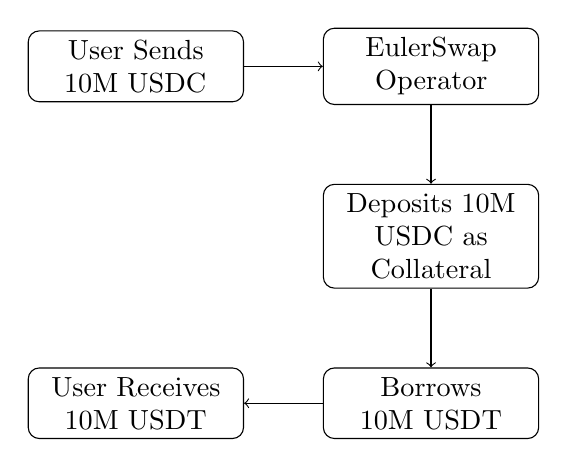
\begin{tikzpicture}[
node distance=1cm,
every node/.style={draw, text width=2.5cm, align=center, rounded corners}
]
% Nodes
\node (user1) {User Sends 10M USDC};
\node (EulerSwap) [right=of user1] {EulerSwap Operator};
\node (deposit) [below=of EulerSwap] {Deposits 10M USDC as Collateral};
\node (borrow) [below=of deposit] {Borrows ~10M USDT};
\node (user2) [left=of borrow] {User Receives 10M USDT};

    % Arrows
    \draw[->] (user1) -- (EulerSwap);
    \draw[->] (EulerSwap) -- (deposit);
    \draw[->] (deposit) -- (borrow);
    \draw[->] (borrow) -- (user2);
\end{tikzpicture}
\caption{\textbf{Swap flow in EulerSwap AMM}. The operator dynamically borrows the output token using the input token as collateral, providing just-in-time liquidity.}
\label{fig:EulerSwap_liquidity}

\end{figure}

\subsection{Liquidation risks}

Borrowing against LP positions or making use of JIT liquidity introduces risks alongside capital efficiency. These positions incur interest on borrowed assets, which can reduce profitability if not offset by swap fees, interest earned on collateral, or external incentives. Moreover, leveraged LPs are vulnerable to liquidation if collateral values drop or debt ratios rise.

JIT is most effective for correlated asset pairs with high LTV ratios, where liquidation risk is minimal. For more volatile asset pairs, LPs can hedge their position externally—for example, using perpetual futures markets, where traders are often paid to hold the short side. A practical strategy could involve deploying a long-only EulerSwap operator while hedging with a short-only position on a perpetuals platform.

\section{Curve mechanics and virtual reserves}

While the operator logic manages execution and capital flow, the behaviour of swaps is ultimately governed by a customisable AMM curve. EulerSwap features a unique curve that allows different amounts of liquidity and different concentrations of liquidity on different sides of the pool based on the reserves available. The space of possible reserves is determined by how much real liquidity an LP has and how much debt their operator is allowed to hold. Since EulerSwap AMMs do not always hold the assets used to service swaps at all times, they perform calculations based on \emph{virtual} reserves and debt limits, rather than on strictly \emph{real} reserves. Each EulerSwap LP can configure independent virtual reserve levels. These reserves define the maximum debt exposure an AMM will take on. Note that the effective LTV must always remain below the borrowing LTV of the lending vault to prevent liquidation. Additionally, different AMM curves influence whether the maximum virtual reserves are achievable.

The EulerSwap curve passes through a reserve equilibrium point $(x_0, y_0)$, at which the marginal price is defined by:

\begin{equation}
\frac{dy}{dx} \Big|_{(x_0, y_0)} = -\frac{p_x}{p_y}.
\end{equation}

Unlike most AMM curves, which are usually defined by a single convex function, EulerSwap uses a piecewise-defined curve, with different functions guiding trading behaviour either side of the equilibrium point. In the domain $0 < x \leq x_0$, the curve is defined by

\begin{equation}
\label{eq:euler-swap-main-y}
y
=
y_{0}+\frac{p_{x}}{p_{y}}\left(x_{0}-x\right)\left(c_{x}+\left(1-c_{x}\right)\left(\frac{x_{0}}{x}\right)\right),
\end{equation}

with $y$ depending on $x$. In the region $x_0 < x$, we let $x$ become the dependent variable, so that the domain is $0 < y \leq y_0$, and the curve is defined by

\begin{equation}
\label{eq:euler-swap-main-x}
x
=
x_{0}+\frac{p_{y}}{p_{x}}\left(y_{0}-y\right)\left(c_{y}+\left(1-c_{y}\right)\left(\frac{y_{0}}{y}\right)\right),
\end{equation}

with $x$ depending on $y$. Although defining an AMM using this technique is unusual, both curves have well-defined inverses, allowing trading behaviour to be fully defined for any swap input or output amount in any direction.

The $c_x, c_y$ parameters in the equations are liquidity concentration parameters that control how liquidity is distributed along the curve, with values closer to 1 concentrating liquidity around the equilibrium point, similar to a Curve StableSwap pool, and values closer to 0 distributing it across a wider price range, similar to a classic Uniswap v2 pool. When the $c$ parameters are both 1, the AMM becomes a constant-sum AMM, and when they are both 0, the AMM becomes a constant-product AMM.

This flexibility enables EulerSwap to be used for entirely new use cases or to simulate the behaviour of atypical AMM protocols, such as the MakerDAO \href{https://mips.makerdao.com/mips/details/MIP29}{Peg Stability Module} (PSM). A full description is given in the Appendix \ref{sec:appendix}.

\begin{figure}[h]
\centering
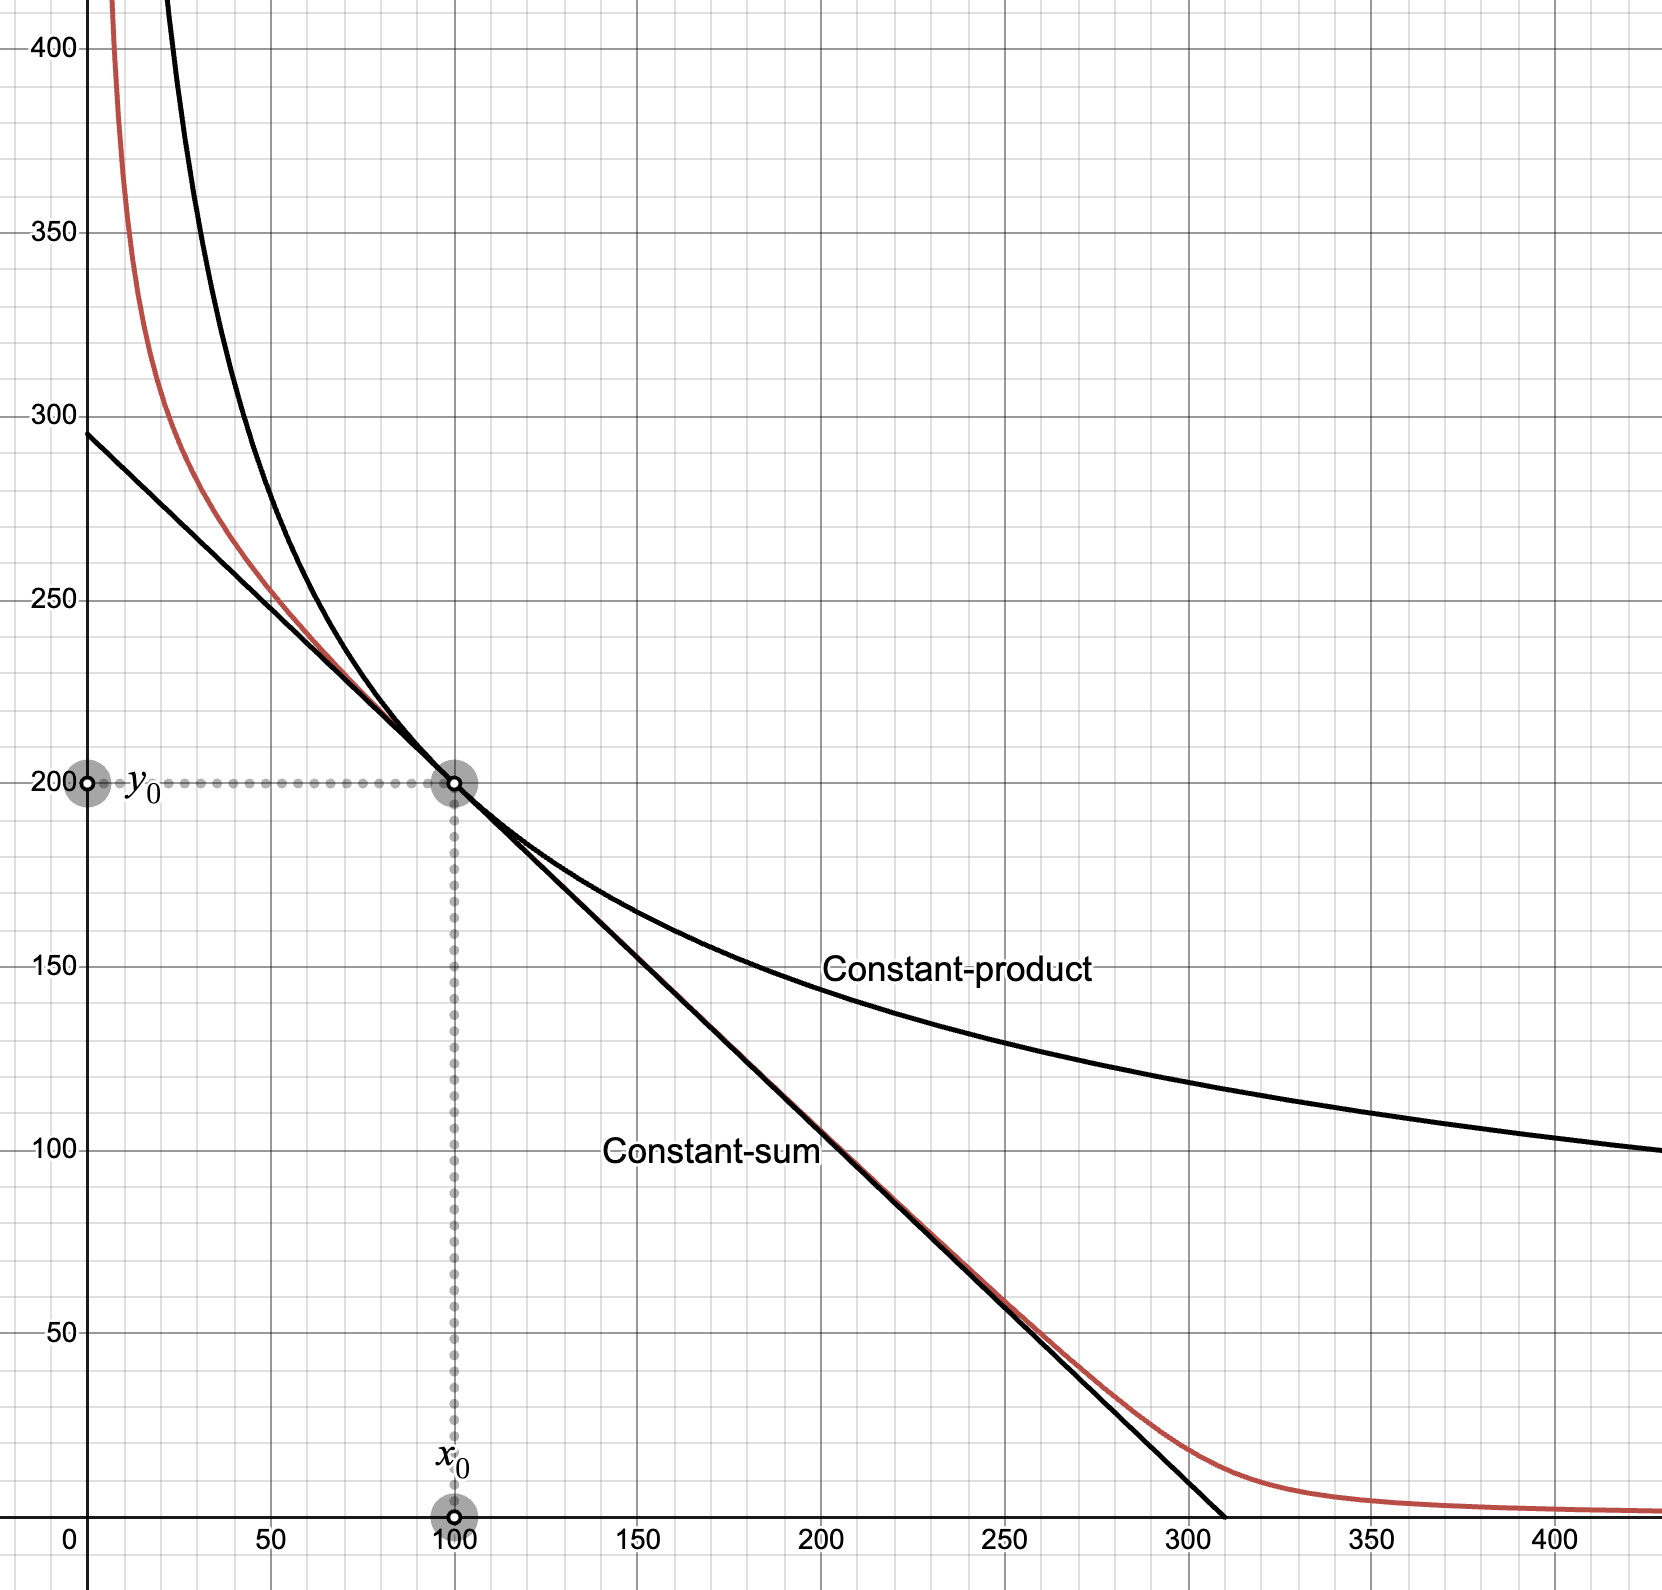
\includegraphics[width=0.5\textwidth]{curve.png}
\caption{\textbf{EulerSwap AMM curve.} The EulerSwap curve (red line) consists of two sides with separate reserve values $x_0, y_0$ and liquidity concentration parameters $c_x, c_y$, allowing liquidity to be distributed asymmetrically. This means liquidity can be more or less dense or concentrated on one side of the AMM relative to the other. The exchange rate at equilibrium is determined by the pricing parameters $p_x, p_y$ and is fully flexible. The curve is also available as an interactive model on \href{https://www.desmos.com/calculator/iczoxr4mhw}{Desmos} to compare its behaviour with traditional constant-sum and constant-product curves (black lines).}
\label{fig:fig1}
\end{figure}

\section{Conclusion}

EulerSwap enhances AMMs by leveraging just-in-time liquidity to expand the depth of liquidity available to swappers. By integrating Euler’s lending vaults, it enables LPs to earn swap fees on top of their ordinary deposits while offering a customisable AMM curve that supports concentrated, distributed, and asymmetric liquidity structures. These features make EulerSwap adaptable to a wide range of trading strategies. By catering to professional market makers, DAOs, and algorithmic trading systems, EulerSwap positions itself as a foundational infrastructure for efficient, programmable on-chain liquidity. 

\section*{Acknowledgments}

During a security review of EulerSwap, Chris Michel noted similarities between some of its underlying concepts and BlackHoleSwap, a project prototype he had reviewed years earlier. While EulerSwap was designed independently and without influence from that project, the resemblance is significant enough to warrant its recognition here as prior art.

\newpage
\section{Appendix}
\label{sec:appendix}

\subsection{Curve description}
\label{sec:curve-description}

Here we describe how the EulerSwap curve generalises the behaviours of both the constant-sum (CSMM) and constant-product market maker (CPMM) curves using liquidity concentration parameters. We begin with an automated market maker (AMM) holding initial liquidity reserves of two assets, $X$ and $Y$, denoted as $x_0$ and $y_0$, respectively. In the absence of trading, the AMM remains at equilibrium at the point $(x_0, y_0)$. 

Our goal is to find a curve for a constant-function trading market maker (CFMM) that supports swaps between the two assets with the following properties:

\begin{itemize}
    \item Passes through the equilibrium point $(x_0, y_0)$.
    \item Maintains an exchange rate, given by the slope of the AMM curve, of $-p_x / p_y$ at $(x_0, y_0)$.
    \item Allows liquidity concentration to be adjusted via parameters $c_x$ and $c_y$, which control the liquidity available for swaps to the left and right of the equilibrium point.
\end{itemize}

To develop such a function, we first introduce two fundamental AMM curve models.

\subsubsection{Constant-sum and constant-product curves}

The canonical CSMM and CPMM curves are given by:

\begin{align}
    x + y &= x_0 + y_0, \\
    xy &= x_0 y_0.
\end{align}

The CSMM is simply a line, whilst the CPMM is a hyperbola. These curves can be thought of as two extremes when it comes to the distribution of liquidity. The CSMM concentrates liquidity at a single exchange rate, whilst the CPMM distributes liquidity across a wide range of different exchange rates. By default, these curves intersect at the equilbirium point $(x_0, y_0)$, where their slopes are:

\begin{align}
    \frac{dy}{dx} &= -1, \\
    \frac{dy}{dx} &= -\frac{y}{x}.
\end{align}

Since real-world markets often operate at variable exchange rates at equilibrium, we introduce custom pricing parameters $p_x$ and $p_y$ to allow flexibility in defining the slope at the equilibrium point:

\begin{align}
    \label{eq:weighted-line}
    p_x x + p_y y &= p_x x_0 + p_y y_0, \\
    \label{eq:exponential-form}
    x^{p_y y_0} y^{p_x x_0} &= x_0^{p_y y_0} y_0^{p_x x_0}.
\end{align}

The CSMM is now a line with a slope parameterised by the ratio of the pricing parameters, whilst the CPMM is now a \textit{weighted} hyperbola. Taking the derivatives of these equations with respect to $x$, we obtain:

\begin{align}
    \frac{dy}{dx} &= -\frac{p_x}{p_y}, \\
    \frac{dy}{dx} &= -\frac{p_x}{p_y} \frac{x_0 y}{y_0 x}.
\end{align}

These results confirm that at equilibrium $(x_0, y_0)$, the slope of both functions is:

\[
\frac{dy}{dx} \Big|_{(x_0, y_0)} = -\frac{p_x}{p_y}.
\]

While this weighted CPMM generalises the constant-product formula to support a customisable price at equilibrium, it introduces significant computational complexity. In particular, the exponential form involves power functions of reserves, which are expensive to compute on-chain in the EVM. As a result, this formulation is not directly implementable in practice. To address this, we construct an alternative using artificial reserves—a design trick that preserves the slope and equilibrium properties while greatly simplifying the functional form.

\subsubsection{Introducing artificial reserves to create a new, simpler curve}

Note that in the interval $0 < x \leq x_0$ swaps should only increase liquidity beyond $y_0$ and deplete $x_0$ liquidity. That is, our trading function in this interval need not depend on the initial amount of $y_0$ liquidity. This suggests that we can split the domain of the AMM curves into two, and replace the real reserve $y_0$ in the interval $0 < x \leq x_0$ with a carefully chosen artificial reserve $y_v$ designed to eliminate the exponential form in the weighted hyperbola. 

Re-arranging equations \eqref{eq:weighted-line} and \eqref{eq:exponential-form} into explicit functions of $y$, we obtain
\begin{align}
    \label{eq:weighted-line-explicit}
    y &= y_0 + \frac{p_x}{ p_y} (x_0 - x), \\
    \label{eq:exponential-form-explicit}
    y &= y_0 \left( \frac{x_0}{x} \right)^{\frac{p_y y_0}{p_x x_0}}.
\end{align}

In this view, it is easy to see that a substitution of $y_0 \rightarrow y_v$, given by

\[
y_v = x_0 \frac{p_x}{p_y}
\]

will eliminate the exponential form in equation \eqref{eq:exponential-form-explicit}. We then have equations

\begin{align}
    y &= \frac{p_x}{p_y} (2x_0 - x), \\
    y &= \frac{p_x}{p_y} \frac{x_0^2}{x}.
\end{align}

Note that simply shifting the curve up or down does not impact the slope or shapes of the curves and therefore has no impact on trading behaviour. Since these curves no longer pass through \( (x_0, y_0) \), we therefore correct them by adding back the difference \( y_0 - p_x / p_y x_0 \). This leads to:

\begin{align}
    y &= y_0 + \frac{p_x}{p_y} (x_0 - x), \\
    y &= y_0 + \frac{p_x}{p_y} (x_0 - x) \left( \frac{x_0}{x} \right).
\end{align}

Taking the derivatives of these equations with respect to $x$, we obtain:

\begin{align}
    \frac{dy}{dx} &= -\frac{p_x}{p_y}, \\
    \frac{dy}{dx} &= -\frac{p_x}{p_y} \left( \frac{x_0}{x} + \frac{x_0(x_0 - x)}{x^2} \right)
    = -\frac{p_x}{p_y} \left( \frac{x_0}{x} \right)^2.
\end{align}

These results confirm that at equilibrium $(x_0, y_0)$, the slope of both functions is:

\[
\frac{dy}{dx} \Big|_{(x_0, y_0)} = -\frac{p_x}{p_y}.
\]

\subsubsection{Unifying into a single curve in the region $0 < x \leq x_0$}

To create a single unified curve, we introduce a liquidity concentration parameter \( c_x \in [0, 1] \) that determines the curve’s convexity:

\begin{itemize}
    \item When \( c_x = 1 \), the AMM functions as a constant-sum AMM.
    \item When \( c_x = 0 \), the AMM behaves as a constant-product-like AMM.
    \item Intermediate values of \( c_x \) create a hybrid trading function, with liquidity that is more or less concentrated around the equilibrium point.
\end{itemize}

This parameterisation leads to the following equation:

\begin{equation}
    \label{eq:EulerSwap-1}
    y = y_0 + \frac{p_x}{p_y} (x_0 - x) \left( c_x + (1 - c_x) \left(\frac{x_0}{x}\right) \right).
\end{equation}

This equation is equivalent to equation \eqref{eq:euler-swap-main-y} in the main text. It is implemented as the function `f()' in Solidity within the `CurveLib.sol' contract. It serves two main purposes:

\begin{itemize}
    \item Swap quoting: Providing quotes for \(y\) given \(x\) in the domain \(0 < x \leq x_0\).
    \item System invariant: Acting as a key invariant within the EulerSwap system (detailed below).
\end{itemize}

The marginal price at anywhere along the curve is given by the derivative, which is given by:

\begin{align}
    \frac{dy}{dx}
    &=
    \frac{p_x}{p_y} \left[ -\left( c_x + (1 - c_x) \left( \frac{x_0}{x} \right) \right) - (x_0 - x) (1 - c_x) \left( \frac{x_0}{x} \right)^2 \right] \\ \nonumber
    &=
    -\frac{p_x}{p_y} \left[ c_x + (1 - c_x) \left( \frac{x_0}{x} \right)^2 \right] 
\end{align}

To function as a complete trading function, equation \eqref{eq:EulerSwap-1} can also be inverted to compute \(x\) given \(y\) in the range \(0 < x \leq x_0\). By rearranging the formula into a quadratic in \(x\), we derive:

\begin{equation}
    \label{eq:EulerSwap-inverse-1}
    c_{x}x^{2} + \left( \frac{p_{y}}{p_{x}} \left( y - y_{0} \right) - \left( 2c_{x} - 1 \right) x_{0} \right) x - \left(1 - c_{x} \right) x_{0}^{2} = 0.
\end{equation}

This is a quadratic equation in $x$ that we can solve for using the classic quadratic formula. The components of a classic solution would be given by:
\begin{align}
    A 
    &= 
    c_x, \\ \nonumber
    B 
    &=
    \frac{p_{y}}{p_{x}} \left( y - y_{0} \right) - \left( 2c_{x} - 1 \right) x_{0}, \\ \nonumber
    C 
    &= - \left(1 - c_{x} \right) x_{0}^{2}. 
\end{align}

With this, our solution for the positive real root is given by:

\begin{equation}
\label{eq:quadratic-formula}
    x
    =
    \frac{-B + \sqrt{B^2 - 4AC}}{2A}.
\end{equation}

In some circumstances, particularly when $B \geq 0$, this form of the quadratic equation is numerically unstable. In Solidity, we therefore sometimes use an alternative form called \href{https://en.wikipedia.org/wiki/Quadratic_formula}{``citardauq'' formula}, which is a rearrangement of equation \eqref{eq:quadratic-formula} to give:

\begin{equation}
\label{eq:citardauq-formula}
    x
    =
    \frac{2C}{-B - \sqrt{B^2 - 4AC}}.
\end{equation}

By re-defining $C = \left(1 - c_{x} \right) x_{0}^{2}$, and noting that $B = -B$ when $B < 0$, we can further simplify these equations to give:

\begin{align}
    \label{eq:Eulerswap-inverse}
    x =
    \begin{dcases}
    \frac{B + \sqrt{B^2 + 4AC}}{2A}, & \text{if } B \leq 0 \\\\
    \frac{2C}{B + \sqrt{B^2 + 4AC}}, & \text{if } B > 0.
    \end{dcases}
\end{align}

This solution is implemented as the function `fInverse()' in Solidity within the `CurveLib.sol' contract. Its main purpose is to provide quotes to swappers. 

\subsubsection{Extending the curve to the $x \geq x_0$ region}

To support swaps where the input token lies in the region , we need a symmetric extension of the trading function to the right-hand side of the curve. Rather than defining a new function from scratch, we reflect the existing function by interchanging the roles of $x$ and $y$. However, this reflection alone is not sufficient: we must also reparameterise the function to use the correct pricing $p_x, p_y$ and concentration $c_x, c_y$ parameters that govern the behaviour of the AMM on the $y$-side of the pool.

This leads us to the following reparameterised version of equation \eqref{eq:EulerSwap-1}:

\begin{equation}
\label{eq:EulerSwap-2}
x = x_0 + \frac{p_y}{p_x} (y_0 - y) \left( c_y + (1 - c_y) \left(\frac{y_0}{y}\right) \right).
\end{equation}

This equation is equivalent to equation \eqref{eq:euler-swap-main-x} in the main text. It provides a pricing function for swaps in which $x$ is given and $y$ is unknown, and where we are in the domain $0 < y \leq y_0$ (which corresponds to $x \geq x_0$).

Importantly, this is not a new curve, but a reparameterisation of the original left-hand side. It shares the same structural form and equilibrium properties but is applied to the opposite side of the pool using flipped arguments and parameters. In practice, this function is implemented using the same Solidity routine (`f()') as equation \eqref{eq:EulerSwap-1}, with the arguments appropriately swapped to match the trading direction. The inverse of this function can be derived analogously by reparameterising equation \eqref{eq:Eulerswap-inverse}.

\subsection{Invariant}
\label{sec:invariant}

In traditional AMM protocols, the curve is typically defined as an implicit function of $y$. For example, the classic Uniswap AMM follows a constant-product equation:

\begin{equation}
    xy = x_0 y_0
\end{equation}

where $x_0$ and $y_0$ are the reserves of the equilbirium point. This equation defines an invariant condition, ensuring that any valid swap must satisfy:

\begin{equation}
    xy \geq x_0 y_0.
\end{equation}

This condition guarantees that after any trade, the product of the new reserves remains at least as large as the initial product, ensuring that swaps cannot drain liquidity from the pool.

Rearranging this condition, we can express the invariant as a lower bound for $y$:

\begin{equation}
    y \geq \frac{x_0 y_0}{x}.
\end{equation}

This means that for any valid trade, the resulting reserve state must lie on or above the AMM curve.  

\subsubsection{Extending the invariant to EulerSwap}

For EulerSwap, we apply a similar principle. Given any reserve state $(x, y)$, we check whether it satisfies an equivalent invariant condition.

From equation \eqref{eq:EulerSwap-1}, for values where \( 0 < x \leq x_0 \), the AMM curve constraint requires a lower bound for $y$:

\begin{equation}
    \label{eq:invariant-x1}
    y \geq y_{0}+\frac{p_{x}}{p_{y}}\left(x_{0}-x\right)\left(c_{x}+\left(1-c_{x}\right)\left(\frac{x_{0}}{x}\right)\right).
\end{equation}

For values where \( 0 < y \leq y_0 \), which is equivalent to \( x > x_0 \), we simply use a lower bound for $x$ instead:

\begin{equation}
    \label{eq:invariant-x2}
    x \geq x_{0}+\frac{p_{y}}{p_{x}}\left(y_{0}-y\right)\left(c_{y}+\left(1-c_{y}\right)\left(\frac{y_{0}}{y}\right)\right).
\end{equation}

These conditions together define the valid liquidity states in EulerSwap, ensuring that the AMM remains balanced while allowing for greater flexibility in liquidity provisioning.

\section{Disclaimer}

This paper is for general information purposes only. It does not constitute investment
advice or a recommendation or solicitation to buy or sell any investment and should not
be used in the evaluation of the merits of making any investment decision. It should not
be relied upon for accounting, legal or tax advice or investment recommendations. This
paper reflects current opinions of the authors and is not made on behalf of Euler Labs or its
affiliates and does not necessarily reflect the opinions of Euler Labs, its affiliates or individuals
associated with Euler Labs. The opinions reflected herein are subject to change without being
updated.

\end{document}
